% 图 8.5 单离子/各向异性能量随角度变化：K sin^2 theta 曲线
\documentclass[tikz,border=5pt]{standalone}
\usetikzlibrary{arrows.meta}
\usepackage{amsmath}
\usepackage{bm}
\usepackage{fontspec}
\setmainfont{Times New Roman}
\begin{document}
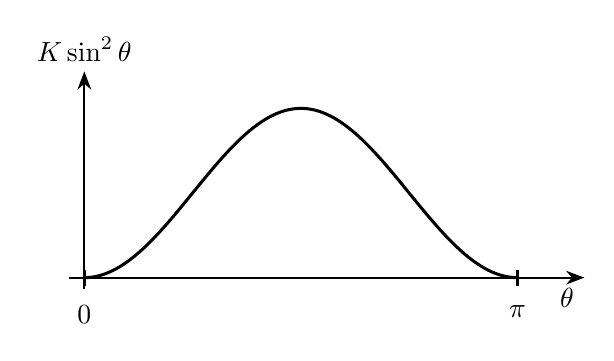
\begin{tikzpicture}[line width=0.8pt,>=Stealth]
  % curve y = K sin^2(theta)
  \draw[line width=1.1,domain=0:180,samples=121,smooth]
    plot ({5.5*\x/180},{2.15*sin(\x)*sin(\x)});
  % axes
  \draw[->] (-0.2,0) -- (6.35,0) node[below left]{$\theta$};
  \draw[->] (0,-0.14) -- (0,2.62) node[above]{$K\sin^2\theta$};
  % tick marks at 0 and pi
  \draw[line width=1.0] (0,-0.10) -- (0,0.10);
  \node[below] at (0,-0.22) {$0$};
  \draw[line width=1.0] (5.5,-0.10) -- (5.5,0.10);
  \node[below] at (5.5,-0.22) {$\pi$};
\end{tikzpicture}
\end{document}
